
We define a multiclass classification problem.\\
Being a multiclass problem it is necessary to use a one-vs-all or all-vs-all method.
In this case we use a linear classifier with an all-vs-all method, in which each class is compared to all the others with each new iteration of the algorithm.\\
We use a $\lambda$ as regularization parameter.
To get the best solution we divide the dataset into two sets: a learning set, corresponding to the $ 70 \% $ of the initial data and a validation set, in order to calculate the error committed by our model, and run a loop on different $\lambda$ values in order to identify the best value.\\
To mediate the result and minimize the influence of variance we repeat this procedure a number k of times, with k equal to 30 for example.
\begin{figure}[h]
	\centering
	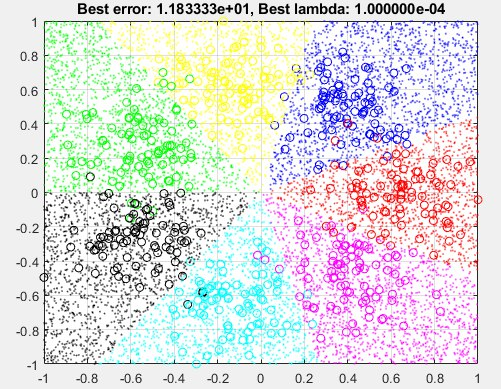
\includegraphics[width=0.5\textwidth]{i1.png}
	\caption{Regression Function}
	\label{fig:regression function}
\end{figure}


